\section{Preliminaries}

\subsection{Trading in Forex}
In first instance, an order is a request to make a trade to open a position.
A trade is made when the order is matched to a counterpart, i.e a buyer has found a seller, or vice versa.
Once a trade is opened, it constitutes a position. A position is exposure to the market and will move the balance in the account up or down in line with market movements. Placing an order to close a position will result in a trade opposite to the direction initially took, e.g. if we initially bought, now we sell to close. When we open a buy position, we are \textit{long}, while when we sell we are \textit{short}.

To be able to start a exchange in Forex, one need to open a position. There are alternatives to open a position: both buying the base currency and selling the quote one (going long) or selling the base one and buying for the quote forex currency (going short). The base and quote currencies are the first and second currencies in a foreign money pair, respectively. For instance, GBP is the base and USD is the quote currencies in GBP/USD forex pair.

A trader can use leverage within the buying and selling. Leverage is the ratio which lets in to trade big amount with a small sum of money. As an instance, if one trades \$ $1000$ with a leverage $1:30$ in GBP/USD, the amount of buying and selling transaction will be \$ $30,000$ instead of \$ $1000$.
The profit or loss of a buying and selling transaction is calculated with the aid of subtracting the final value from the initial price of the foreign money pair. Assume the trader goes long  \$ $30,000$ in GBP/USD with a buying price of $1.4060$ and closes his position with a selling price of $1.4090$. The difference is $0.0030$ equals to 20 pips. Due to the fact the initial position is long and price went up, the transaction is profitable and the earnings is $30,000 * 0.0030 =$ \$90. Consequently the trader wants the price of the forex pair to growth whilst he/she is long and decrease when he/she is short to be able to get profit.

\subsection{Trading System: Meta Trader 5}
Since its introduction in 2005, MetaTrader 4 has become the most popular trading platform in the Forex world. It is supported by dozens of brokers worldwide, and offers traders the ability to program custom trading systems and indicators in the MQL language. The wide adoption of MetaTrader Forex brokers has created a large worldwide community of users.

In 2010 MetaQuotes launched the public beta of MetaTrader 5. The new platform introduces support for additional financial instruments, including futures and stocks. A one-click trading interface allows you to open orders quickly. Charts now support custom periods. For discretionary traders, MetaTrader 5~\footnote{https://www.metatrader5.com/en/trading-platform}  has a built-in news calendar and a wide variety of chart objects, including Elliott, Gann and Fibonacci tools.

But the biggest change in MetaTrader 5 has been the new MQL5 programming language. The latest version of MQL has been rebuilt from the ground up as a modern object-oriented programming language. Many new features have been added, including new data types, events, chart operations and more. The redesign of MQL5 also means that it is a much different language than MQL4. MQL5 is much more powerful and efficient than its predecessor~\cite{young13}. 

We used MQL5 to implement an \textit{expert advisor} that is an automated trading program that can open, modify and close orders. The end goal of our research is to provide to the community the implemented expert advisor~\footnote{https://git.l3s.uni-hannover.de/mfisichella/forex}, which was developed using the MetaEditor as IDE (Integrated Development Environment) for MQL5, included in Metatrader 5, and extending the shared code written by Young~\footnote{http://www.expertadvisorbook.com/MQL5BookSourceCode.zip} . 

\subsection{Technical indicators}
Technical analysis is the observation of past market motion with the scope to forecast future prices and to deal with the effect of the market movement. Two are the main approaches considered in this analysis. Based on charts, the analysis tends to detect patterns in price charts. There are 4 main types of charts used by traders: Bar chart, line chart, candlestick chart and point and figure chart. We use Candlestick chart.

The candlestick is a type of graphical representation of the prices in the time, similar to the Bar chart but is of easier reading.

\begin{figure}[h]
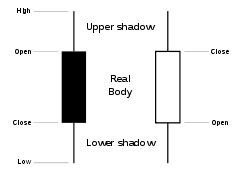
\includegraphics[scale=0.5]{candle}
\centering
\caption{Candlesticks.}
\label{fig:candle} 
\end{figure}

In Fig.~\ref{fig:candle} are represented some characteristics of the candlestick: first of all we notice the colour of the said Real Body, that it identifies the amplitude of the price between the opening and the closing, then two connected appendices called shadows and therefore upper shadow for that advanced and lower shadow for that inferior.

A candlestick with a closing price higher than the opening one is called \textit{Bullish} and it has \textit{white} colour, while \textit{black} for those ones with a closing price lower than the opening one, called \textit{Bearish}.

The Candlestick charts form in the time pattern that are identified according to the amplitude of the body, according to the conformation and the succession of candles or groups of candles~\cite{OZTURK2016170}.

It is well to notice that when the lower shadow is particularly long, the probabilities of reversal increase, the candle assumes one strong connotation of reversal. In fact, more long they are the shadows, greater it is the sense of instability of the market and more probable will be the signal of reversal.


In our trading system, 20 technical indicators are used as the basis of trading rules. These technical indicators are: Adaptive Moving Average, Average Directional Moving Index, Donchian channel, Stoller Bands, Bollinger Bands, Double Exponential Moving Average, Envelope Moving Avarage, Parabolic SAR, Fractal Adaptive Moving Avarage, Standard Deviation, Triple Exponential Moving Average, Avarage True Range, Bears Power, Bulls Power, MACD (Moving Average Convergence Divergence), Stochastic oscillator, William' Percentage Range, Momentum, RSI (Relative Strength Index), and Heiken Ashi Candles.

\subsection{Trading Rules}


\subsubsection{Trading Rules with Dynamic Channels}
Many operating strategies built for short-term trading use signals provided by what are known in technical jargon as 'dynamic channels'. In some cases the strategies are of type trend following, that is they aim to follow the main trend present on the market, in other cases instead they are of type reversal in how much they try to take advantage of a possible reversal of trend.
The principle of base of these operating techniques is based on the individualization of some bands of oscillation (envelopes) that:

\begin{itemize}
\setlength\itemsep{0.3em}
\item Contain for the greater part of the time the movement of the prices.
\item They concur to characterize the trend followed from the prices.
\item They supply interesting reversal signals.
\end{itemize}

These channels are dynamic in how much, measuring (even if in various way) the present instability on the market, they are adapted to the movements (cyclical) carried out from the prices, that alternate in fact phases of consolidation (in which the instability is reduced) to directional/impulsive phases (in which the instability increases in meaningful way). The technique of the bands requires the identification of:

\begin{itemize}
\setlength\itemsep{0.3em}
\item A central reference average, which serves to identify and exploit the primary trend present in the market;
\item A lower band and an upper band, which constitute respectively a support and a resistance of dynamic type (as they move according to the volatility recorded on the market) and which contain the movement of prices.
\end{itemize}

When volatility is low the two bands narrow and approach prices (the channel width is reduced), when volatility is high the two bands widen and move away from prices (the channel width increases). 

We begin therefore with the description of the more used dynamic channels, beginning from the Channel of Donchian and the Bands of Stoller. 

\paragraph{\textbf{Donchian channel}}\mbox{}

One of the first operational techniques based on the use of channels was invented by Richard Donchian who built a trend following system based on the identification of the highs and lows of the last 20 days (the original system was based on the \textit{Donchian 4-week rule}). With this technique:

\begin{itemize}
\setlength\itemsep{0.3em}
\item Long positions were opened when prices exceeded the highest high of the last 20 days.
\item One would open short positions when they fall below the lowest low of the last 20 days.
\end{itemize}  

With this technique one goes in search of the classic breakout signals that can initiate a directional movement. Draft however of a system that has been applied with success during the years $'80$ on the market of the commodities (where the tendencies were stable and consisting) but that in the course of the time has diminished its efficiency. For this reason it has been gone to the search of techniques in a position to exploiting also the frequent and unexpected reversals of tendency that are verified when the prices catch up important zones of resistance and/or support.

\paragraph{\textbf{Stoller Bands}}\mbox{}

An experienced commodities trader, Manning Stoller, has constructed an operating technique (Stoller Average Range Channels, STARC) which uses the concept of the Average True Range (ATR). This differs from the simple daily range (the difference between the high and the low price) in that it also takes into account whether there is a gap-up or gap-down.
The ATR is the greater of these three differences:

\begin{itemize}
\setlength\itemsep{0.3em}
\item Today's maximum price minus today's minimum price.
\item Today's maximum price minus yesterday's closing price.
\item Yesterday's closing price minus today's low price.
\end{itemize}  


To calculate the Stoller Bands, a 6-period moving average is calculated, to which the 15-period moving average of the Average True Range multiplied by two is added (to obtain the upper band) and subtracted (to obtain the lower band).
There are therefore three reference lines:

\begin{itemize}
\setlength\itemsep{0.3em}
\item The Upper Band equals to the 6-period moving average plus $(ATR*2)$.
\item The Central Average equals to the 6-period moving average.
\item The Lower Band equals to the 6-period moving average minus $(ATR*2)$.
\end{itemize}  


The difference from the technique proposed from Donchian (of trend following type), the Stoller Bands come used in order to obtain of the signals of reversal. In particular:

\begin{itemize}
\setlength\itemsep{0.3em}
\item Short signals are obtained when prices go beyond the upper band and draw a reversal short bar (for example a shooting).
\item Long signals are obtained when the prices come down under the inferior band and draw a bar of reversal long (as an example a hammer).
\end{itemize} 

\paragraph{\textbf{Bollinger Bands}}\mbox{}

Bollinger Bands are composed of three lines: a central moving average and two bands, one upper and one lower, which automatically widen and narrow according to the volatility expressed by the market. The calculation of Bollinger Bands, according to the original formula of its creator, is simple: 

\begin{itemize}
\setlength\itemsep{0.3em}
\item The value of the upper band is obtained by adding to the central moving average (e.g. at 20 periods) the value of the standard deviation multiplied by two. 
\item The lower band is obtained by subtracting the standard deviation multiplied by two from the moving average (e.g. at 20 periods). 
\end{itemize} 

In this way, when the market is moving sideways, volatility is reduced and the two bands compress around prices. When the market is in a directional phase (either positive or negative), volatility increases and the two bands move away from the prices.

The strategies that can be constructed with the Bollinger Bands are substantially two:\\

\noindent\textit{1. The volatility breakout.} When the bands are compressed around the prices, it means that on the market a marked contraction of the volatility has been verified, situation that can anticipate the beginning of an impulsive movement that often is born with a bar of breakout bullish or bearish. In this case it can be constructed a strategy of trend-following type, time to exploit the trend bullish or bearish that is established thanks to the breakout. For example:

\begin{itemize}
\setlength\itemsep{0.3em}
\item A long position can be opened when prices, following a breakout, accelerate to the upside and push beyond the upper band. The signal must be confirmed by both a close of the candle which is above the upper band and the next candle, which must not be bearish.
\item A short position can be opened when prices, following the breakout, fall rapidly and fall below the lower band. The signal is confirmed both by a close of the candle which is below the lower band and by the next candle which must not be bullish. 
\end{itemize} 

This is an interesting strategy from a theoretical point of view, but it can result in a late entry into the market, with prices having already made a significant movement.\footnote{In order to use signals of breakout it is preferable to use the Channel of Keltner, much more rapid in signalling the beginning of a directional trend.}  \\

\noindent\textit{2. The signals of reversal.} The second technique is of reversal and is that one that is preferred, in how much it exploits the exhaustion of a movement to the rise or the end of a trend negative, and is based on the individualisation of a configuration of reversal, that it is verified when the prices are carried to contact of one of the two bands: 

\begin{itemize}
\setlength\itemsep{0.3em}
\item A bearish signal occurs when the market rips to the upside, crosses the upper band (the upper shadow of the first candle is above the upper band), but then prices undergo a correction and return just below the band itself and the next session draws a bear candle.The signal can be strengthened demanding that the Slow Stochastic gives a short signal (with the line \%K that, inside the area of iper-bought, crosses from the high towards the bottom the line \%D).
\item A bullish signal is had when the market accuses one brusca decrease, comes down under the inferior band (the first candle has one lower shadow under the inferior band), but then the prices bounce and return endured over the same band and draw one second candle bull.The signal can be strengthened demanding that the Slow Stochastic supplies one signal long (with the line \%K that, inside the area of iper-sold, crosses from the bottom towards the high the line \%D).
\end{itemize} 
